% !TEX TS-program = pdflatexmk

\documentclass[modern]{aastex61}
\usepackage[utf8]{inputenc}
\usepackage{hyperref}
\usepackage{natbib}
\usepackage{graphicx}
\usepackage{xspace}
\usepackage{amsmath}
\usepackage{amssymb}

\include{macros}
% Journals


% Astronomical abbreviations (thanks to Dan Huber)
\newcommand{\numax}{\mbox{$\nu_{\rm max}$}\xspace}
\newcommand{\Dnu}{\mbox{$\Delta \nu$}\xspace}
\newcommand{\dnu}{\mbox{$\delta \nu$}\xspace}
\newcommand{\muHz}{\mbox{$\mu$Hz}\xspace}
\newcommand{\teff}{\mbox{$T_{\rm eff}$}\xspace}
\newcommand{\logg}{\mbox{$\log g$}\xspace}
\newcommand{\feh}{\mbox{$\rm{[Fe/H]}$}\xspace}
\newcommand{\msun}{\mbox{$\mathrm{M}_{\odot}$}\xspace}
\newcommand{\mearth}{\mbox{$\mathrm{M}_{\oplus}$}\xspace}
\newcommand{\rsun}{\mbox{$\mathrm{R}_{\odot}$}\xspace}
\newcommand{\kepler}{\emph{Kepler}\xspace}
\newcommand{\hipparcos}{\emph{Hipparcos}\xspace}
\newcommand{\gaia}{\emph{Gaia}\xspace}
% \newcommand{\ktwo}{\textit{K2}\xspace}
\newcommand{\ktwo}{\emph{K2}\xspace}
\newcommand{\ksc}{{\sc k2sc}\xspace}
\newcommand{\ksf}{{\sc k2sff}\xspace}
\newcommand{\kms}{\,km\,s$^{-1}$} % kilometres per second
\newcommand{\bibtex}{\textsc{Bib}\!\TeX} % bibtex. Not quite the correct typesetting, but close enough


\begin{document}

\title{Detection of Oscillations in Aldebaran with Ground-Based Observations}

\author[0000-0003-1540-8562]{Will M. Farr} 

\affiliation{Birmingham Institute for Gravitational Wave Astronomy,
  University of Birmingham, Birmingham, B15 2TT, United Kingdom}

\affiliation{School of Physics and Astronomy, University of
  Birmingham, Birmingham, B15 2TT, United Kingdom}

\author{Guy R. Davies}

\affiliation{School of Physics and Astronomy, University of
  Birmingham, Birmingham, B15 2TT, United Kingdom}

\author[0000-0003-2595-9114]{Benjamin J. S. Pope}
\affiliation{Sydney Institute for Astronomy, School of Physics, University of Sydney, Sydney NSW 2006, Australia} 
\affiliation{Center for Cosmology and Particle Physics, Department of Physics, New York University, 4 Washington Place, New York, NY 10003, USA}
\affiliation{NASA Sagan Fellow}

\author{Thomas North}
\affiliation{School of Physics and Astronomy, University of Birmingham, Birmingham, B15 2TT, United Kingdom}

\author{James Barrett}
\affiliation{Birmingham Institute for Gravitational Wave Astronomy,
  University of Birmingham, Birmingham, B15 2TT, United Kingdom}

\affiliation{School of Physics and Astronomy, University of
  Birmingham, Birmingham, B15 2TT, United Kingdom}

\email{w.farr@bham.ac.uk, G.R.Davies@bham.ac.uk, b.pope@sydney.edu.au, txn016@student.bham.ac.uk, jimbarrett27@gmail.com}

\begin{abstract}
Stuff.
\end{abstract}

\section{Introduction}

Aldebaran, or $\alpha$~Tauri, is a well-known first-magnitude naked-eye red giant star, and has long been the subject of astronomical investigations. Following the proposal of \citet{struverv} several groups began to search for planets by the radial velocity (RV) method, looking for Doppler shifts from the star's reflex motion around the common centre of mass, culminating in the discovery of 51~Peg~b \citep{51peg}, the first exoplanet to be recognized as such. Before this, \citet{hatzes1993} noted RV variations in Pollux \citep[$\beta$~Gem; subsequently confirmed as a planet:][]{betgemconf,betgemconf2}, Arcturus ($\alpha$~Boo, unconfirmed), and Aldebaran. After further investigation by \citet{Hatzes1998}, \citet{Hatzes2015} now claim a firm RV detection of a planetary-mass companion Aldebaran~b, with a period of $628.96 \pm 0.90$~d. 

In this paper, we present a re-analysis of these original RV data in which we not only confirm this signal, but detect acoustic oscillations in Aldebaran for the first time. We validate this method and its result with new RV observations with the SONG~Telescope, and photometry from the \ktwo Mission. By measuring the average frequency \numax of these \emph{p}-mode oscillations we asteroseismically determine the mass of Aldebaran to be $1.17 \pm 0.05$~\msun. This measured stellar mass allows us to calculate that any moons of this giant planet, although they are now likely to be very hot, may have had equilibrium temperatures comparable to that of the Earth when Aldebaran was on the main sequence, raising the possibility that tehy may have once been habitable.

Our new approach to asteroseismic data analysis, based on Continuous Auto-Regressive Moving Average (CARMA) models, can extract exoplanet signals together with measures of \numax from sparse and irregularly-sampled time series. An all-sky survey planetary companions to precisely measure the masses of all nearby red giant stars is feasible with this new approach, and the required data either already exist in large exoplanet surveys, or are easy to obtain with ground-based telescopes.

\section{Time-Domain Models}

It is easy to observe Aldebaran and similarly-bright stars with ground-based spectroscopic instruments, typically only requiring short exposures that can be obtained even under adverse observing conditions. There is indeed a considerable archive of such observations already, as a legacy of radial velocity (RV) surveys conducted to find exoplanets. In most cases, however, these have not so far been useful for asteroseismology, because these RV data are sparsely and irregularly-sampled. Because we have to pause observations during the day, during poor weather conditions, or simply when targets of higher priority are being observed, we get time series of only a few points and which may have significant and uneven gaps. This introduces a window-function effect: the power spectrum as constructed for example by a Fourier transform, or a Lomb-Scargle Periodogram \citep{lomb,scargle}, is convolved with the Fourier transform of the window function, introducing strong sidelobes adjacent to real frequency peaks and causing crosstalk between adjacent frequency channels. This imposes significant limitations both on the signal-to-noise and frequency resolution of power spectra derived from linear methods such as the Lomb-Scargle periodogram, and in practice makes asteroseismology difficult or impossible from the ground for stars with oscillation frequencies ranging from $\sim 12$~h to $\sim$~a few days. 

If we apply nonlinear statistical inference methods...

Reference \citet{Kelly2014}, compare to \citet{Foreman-Mackey2017}.

\section{Aldebaran}
Aldebaran is a red giant star with spectral type K5, one of the nearest such stars at a distance of only $19.96 \pm 0.38$~pc \citep{hipparcos}. Its position near the Ecliptic permits the determination of its angular diameter by lunar occultations and by interferometry \citep[$20.58 \pm 0.03$ mas;][]{richichi2005,1979ApJ...228L.111B,brown1979,panek1980}.

\subsection{SONG Observations}

\subsection{K2 Observations}

In order to verify the results of the novel analysis presented above, we sought to obtain an independent detection of the oscillations of Aldebaran and compare the frequencies determined with the two methods. 

Aldebaran was therefore observed with \ktwo under Guest Observer Program 130471 in Campaign~13, from 2017-03-08 to 2017-05-27. The \kepler Space Telescope \citep{2010sci...327..977b}  
suffered a critical reaction wheel failure in May 2013, which made it impossible to maintain a stable pointing and therefore continue its nominal mission. It was revived as \ktwo \citep{howell14}, balanced by orienting perpendicular to the Sun. This requires that \ktwo observes fields in the Ecliptic in $\sim~80$~d Campaigns. 

As Aldebaran is extremely bright, it saturates the \kepler detector and it is therefore not possible to use standard photometry pipelines to extract a K2 lightcurve. We therefore use halo photometry \citep[as originally implemented in]{White2017}, whereby unsaturated pixels from the outer part of the large and complicated halo of scattered light around bright stars are used to reconstruct a light curve. The brightness of this halo varies in the same way as that of the primary star, and we therefore obtain data in a region of 20~pixel radius around the mean position of Aldebaran, and discard saturated pixels. We construct our halo light curve as a weighted linear combination of individual pixel-level time series, as described in Appendix~\ref{halo}. We then additionally correct the halo light curve using \textsc{k2sc} \citep{k2sc}, though we find that this has a minor effect. There is somewhat higher than usual residual noise at multiples of $4 c/d$ (the satellite thruster firing frequency), but this is nevertheless very small in comparison to the signal from Aldebaran, and may be ascribed to the large fraction of the pixel mask occupied by the bleed column from this extremely bright star.

Using the \textsc{k2ps} planet-search code \citep{k2ps,Pope2016} to examine this light curve, we search for transits across a wide range of periods, and find no evidence either of planetary transits or an eclipsing stellar companion.

\begin{figure}
\centering
% 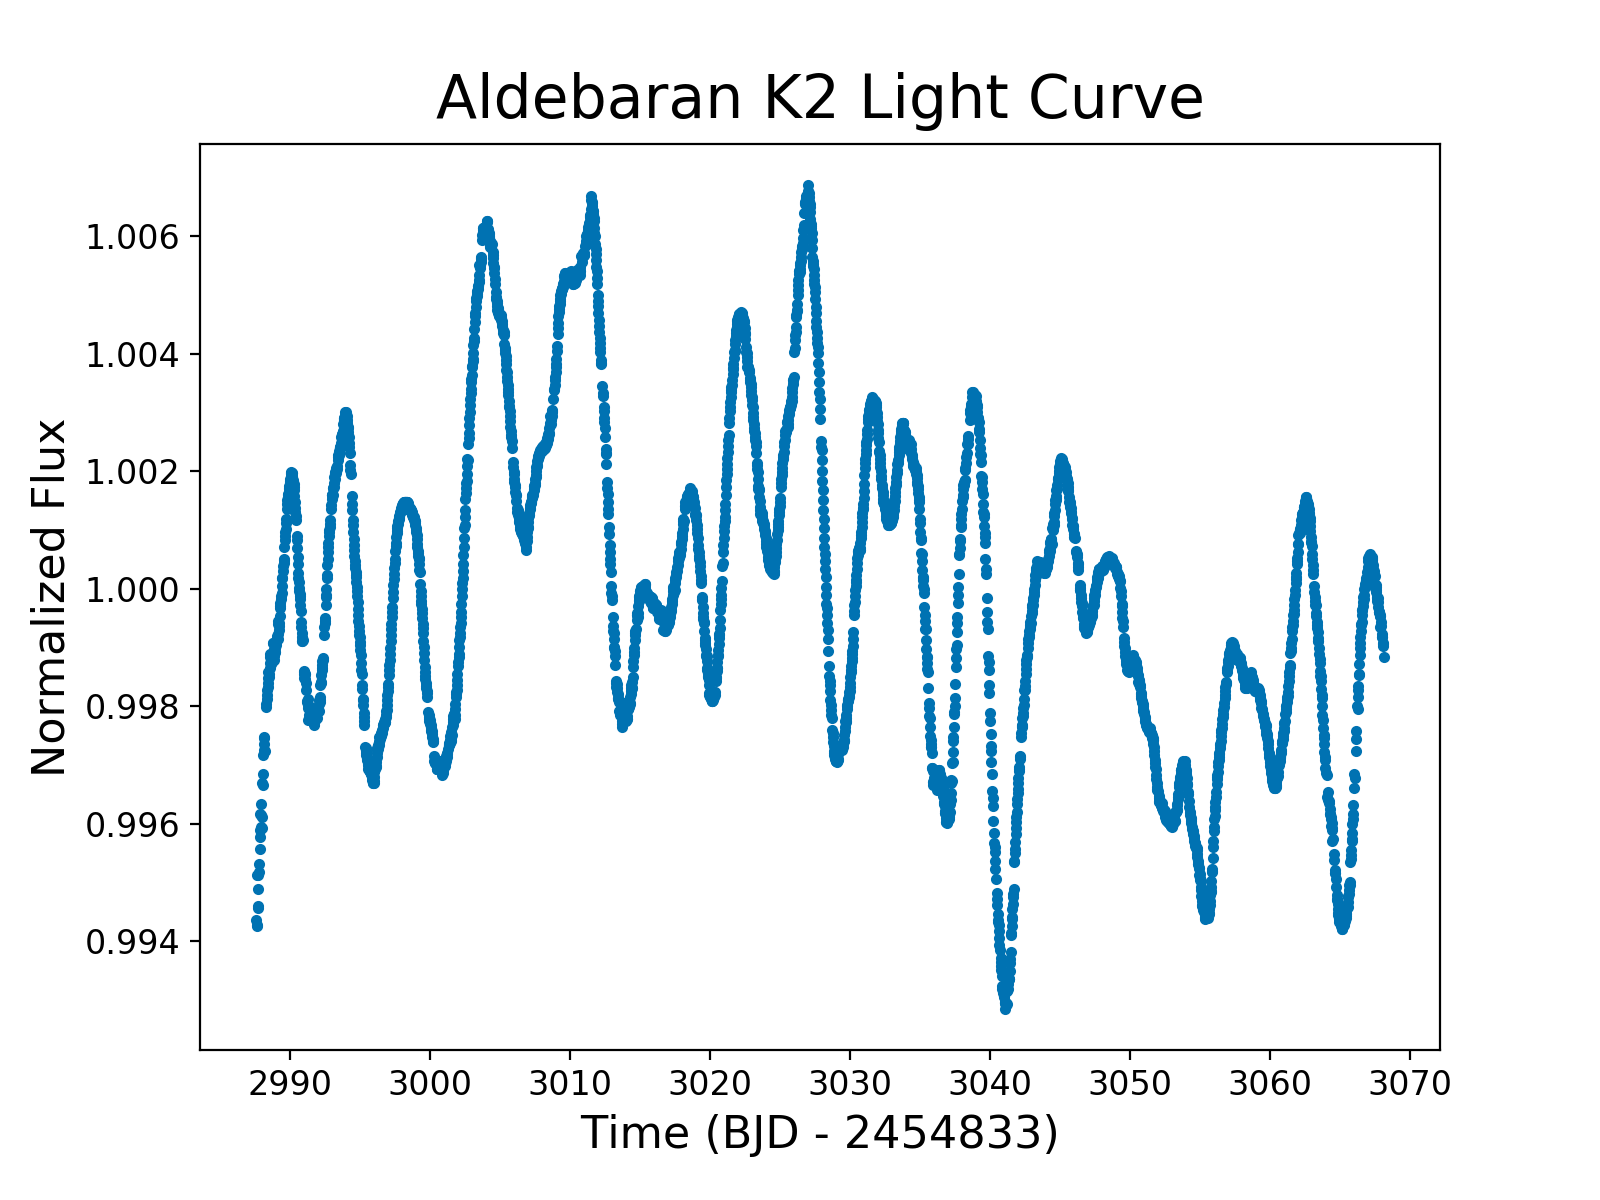
\includegraphics[width=0.75\textwidth]{Aldebaran_lc.png}
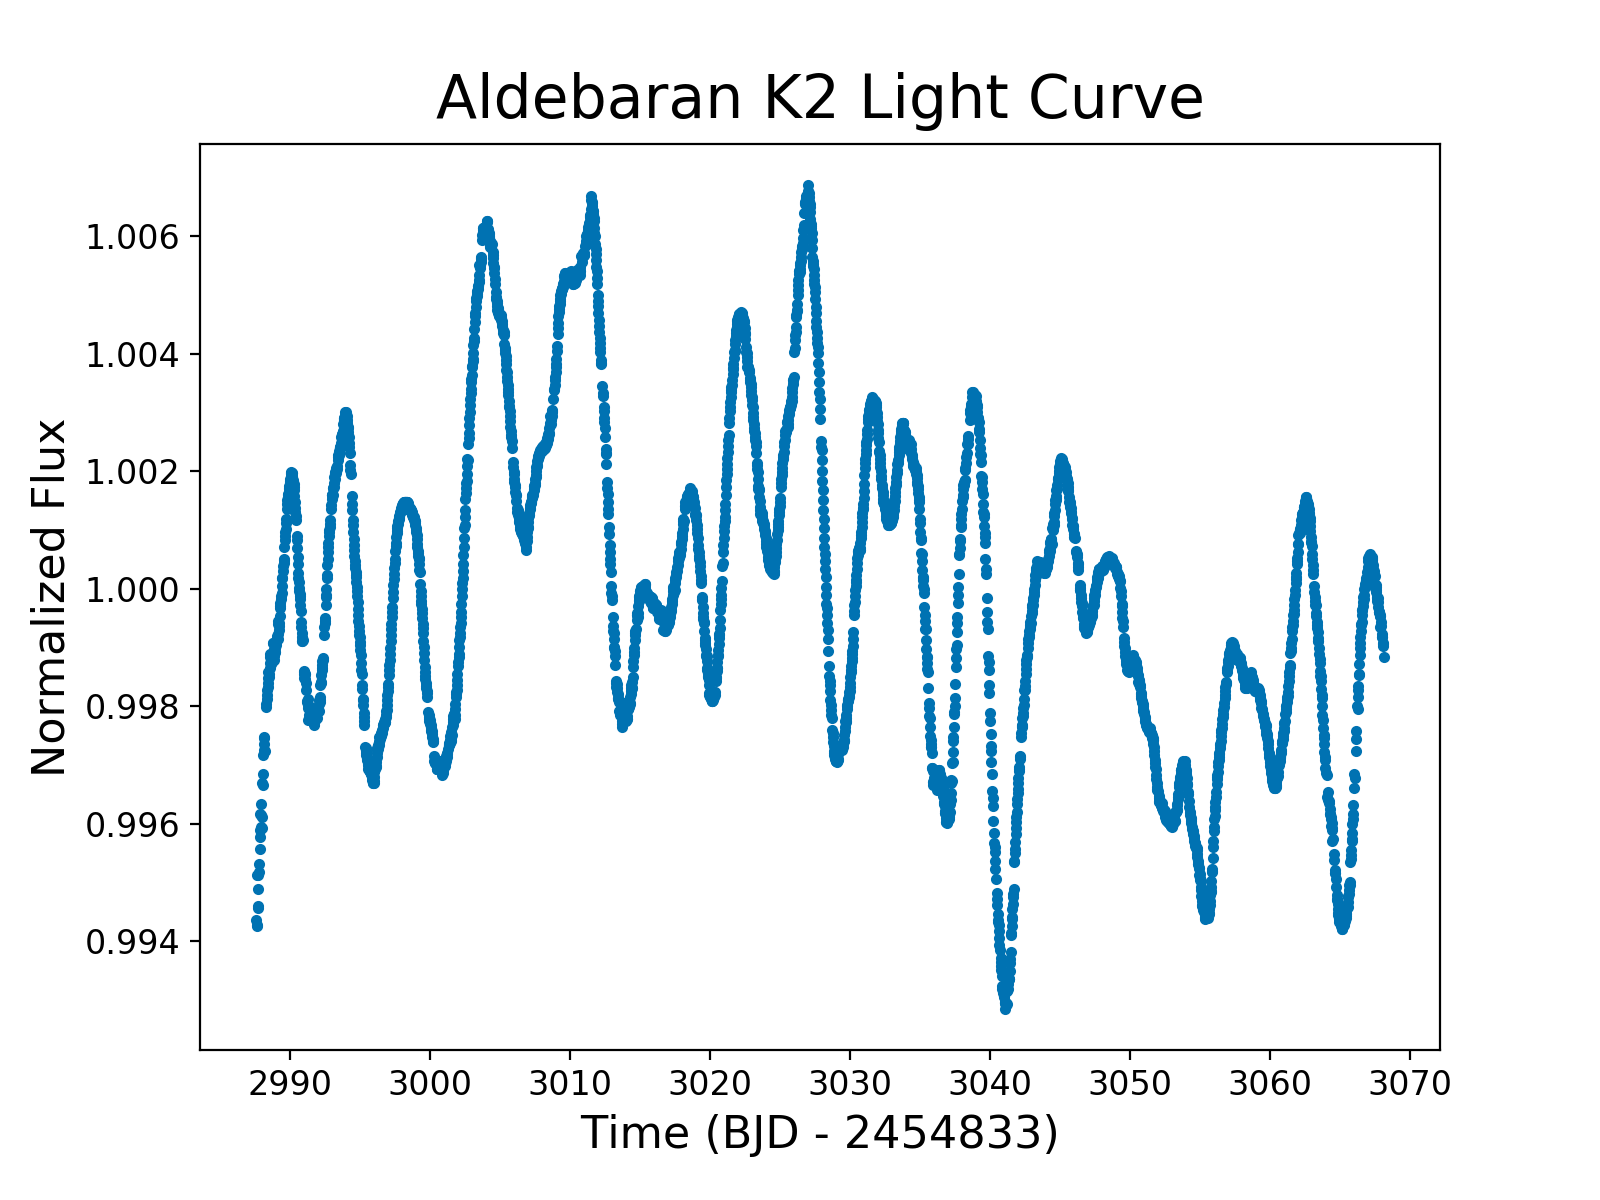
\includegraphics[width=0.75\textwidth]{Aldebaran_lc.eps}
\caption{\ktwo lightcurve of Aldebaran.}
\label{k2_lightcurve}
\end{figure}

\subsection{Stellar Parameters}

\section{Conclusions}

\acknowledgments

We thank the academy....

BP is grateful for funding from the Breakthrough Prize Foundation. This work was performed in part under contract with the Jet Propulsion Laboratory (JPL) funded by NASA through the Sagan Fellowship Program executed by the NASA Exoplanet Science Institute.

This research has made use of the SIMBAD database, operated at CDS, Strasbourg, France, and NASA's Astrophysics Data System. The \kepler data presented in this paper were obtained from the Mikulski Archive for Space Telescopes (MAST). STScI is operated by the Association of Universities for Research in Astronomy, Inc., under NASA contract NAS5-26555. Support for MAST for non-HST data is provided by the NASA Office of Space Science via grant NNX13AC07G and by other grants and contracts.  This work made use of the \textsc{IPython} package \citep{PER-GRA:2007}; SciPy \citep{scipy};  \textsc{matplotlib}, a \textsc{Python} library for publication quality graphics \citep{Hunter:2007}; \textsc{Astropy}, a community-developed core \textsc{Python} package for astronomy \citep{2013A&A...558A..33A}; and \textsc{NumPy} \citep{van2011numpy}. Some of the acknowledgements were compiled using the Astronomy Acknowledgement Generator.

\appendix

\section{Halo Photometry}
\label{halo}

The \kepler detector saturates for stars brighter than the $\sim~11^\text{th}$ magnitude. Nevertheless, the excess flux deposited in a saturated pixel spills conservatively up and down the pixel column, such that it is possible to sum this `bleed column' for bright stars and still obtain precise photometry, such as was done for the brightest star in the nominal \kepler mission, $\theta$~Cyg \citep{guzik2011,thetacygwhite,guzik2016} ($V = 4.48$). There are two main reasons why this is not possible for all bright stars in general. First, because the downlink bandwidth from \kepler is very limited, it is often not desirable to download the large pixel stamps as are required for such bright stars; these must be even larger in \ktwo to account for the reduced image stability. Second, if the bleed column for a sufficiently bright star reaches the edge of the chip, flux spills over and is not conserved, imposing a hard brightness limit that depends on the distance to the detector edge. 
Collateral `smear' data, which are collected to help calibrate the photometric bias from stars sharing the same column as a target, can be used to reconstruct light curves for un-downloaded bright stars and thereby avoid bandwidth constraints \citep{k2smear}, but these data are still rendered unusable if the bleed column falls off the edge of the chip and contaminates the smear rows.

Bright stars have a wide, complicated, position-dependent point spread function (PSF) arising from diffraction and scattering from secondary and higher-order reflections inside the instrument, with the result that they may contaminate thousands of nearby pixels with significant flux. We can therefore use this `halo' of unsaturated pixels for photometry. In this paper we proceed as in \citet{White2017}, in which the method was demonstrated on the seven bright Pleiades, with only minor changes.

The flux $f_i$ at each cadence $i$ is constructed as a weighted sum of pixel values $p_{ij}$:

\begin{equation}
	f_i = \sum_{j=1}^{M} w_j p_{ij}.
\end{equation}

\noindent We choose the weights $w_j$ such that they lie between 0~and~1, add to unity, and minimize the Total Variation (TV) of the weighted light curve. In the continuous case, $n$-th order TV is defined as the integral of the absolute value of the $n$-th derivative of a function; in the discrete case, replacing the derivative with finite differences, first-order TV becomes

\begin{equation}
\text{TV} = \dfrac{\sum_{i=1}^{N} |{f}_i - {f}_{i-1}|}{\sum_{j=1}^{N} {f}_j}
\end{equation}

\noindent and likewise second-order TV the equivalent expression in second-order finite differences. 

In an improvement since \citet{White2017}, we use the \textsc{Theano} library \citep{theano} to calculate analytic derivatives for this objective function, which reduces the computational time for a single halo light curve on a commercial laptop from tens of minutes to tens of seconds. 

As a final step to reduce residual uncorrected systematics, we apply the \textsc{k2sc} \citep{k2sc} Gaussian Process-based systematics correction code to the initial halo light curve, but the effect of this in the present case for Aldebaran is minimal.

\bibliography{aldebaran}



\end{document}